\documentclass[12pt]{article}

\setlength{\parindent}{0pt}
\setlength{\parskip}{2mm}

\usepackage{geometry}
 \geometry{
 letterpaper, left=20mm, right=20mm,  top=20mm,
 }
\usepackage{graphicx}
\graphicspath{ {graphics/} }
\usepackage{amssymb}
\usepackage[hidelinks]{hyperref}
\usepackage{wrapfig}
\usepackage[margin=1.2cm]{caption}
\usepackage{intcalc}


%%%%%%%%%%%%%%%%%%% TIKZ CUSTOM SHAPES AND SETTINGS
\usepackage{tikz}
\usetikzlibrary{shapes.geometric, arrows, positioning, automata}
\usetikzlibrary{calc}
\usetikzlibrary{matrix}
\usetikzlibrary{topaths}
\usetikzlibrary{intersections}
\tikzstyle{device} = [rectangle, rounded corners, minimum width=3cm,
	minimum height=1cm,text centered, draw=black]
\tikzstyle{arrow} = [thick,->,>=stealth]
\tikzstyle{transducer} = [draw,circle,minimum size=1cm,inner sep=0pt]
\tikzstyle{pin} = [draw,circle,radius=5mm,fill=yellow,font=\scriptsize]

\tikzset{wire board/.style={matrix of nodes,
                            row sep=2mm,
                            nodes={anchor=center}
                            },
        rx/.style={column 1/.style={nodes={left}},
                                       column 3/.style={nodes={above right}},
                                       column 2/.style={font=\bfseries}
                                       },
        pi/.style={column 1/.style={nodes={left}},
                                       column 3/.style={nodes={above right}},
                                       column 2/.style={font=\bfseries}
                                       },
        arduino/.style={column 1/.style={nodes={above left}},
                                       column 3/.style={nodes={right}}
                                       }
}
%%%%%%%%%%%%%%%%%%%%%%%%%%%%%%%%%%%%%%%%%%%%%%%%%%%%%%%%%%%%%%%%%%%%%%%%%%%%%%%


%%%%%%%%%%%%%%%%%%% GLOSSARY
\usepackage[toc]{glossaries}
\makeglossaries

% Display 'full' version on first use and short version on subsequent uses
\setacronymstyle{long-short}

\newglossaryentry{hydrophone}
{
	name=hydrophone,
	description={An underwater microphone}
}

\newglossaryentry{iCRAB-proto}
{
	name={iCRAB Transmission Protocol},
	description={Our custom encoding protocol for transmitters.
		See Reference \ref{ref-icrab-proto} for complete documentation}
}

\newacronym{spi}{SPI}{Serial Peripheral Interface}
\newacronym{i2c}{I$^2$C}{Inter-Integrated Circuit}
\newacronym{gpio}{GPIO}{General Purpose Input Output}
\newacronym{pcb}{PCB}{Printed Circuit Board}
%%%%%%%%%%%%%%%%%%%%%%%%%%%%%%%%%%%%%%%%%%%%%%%%%%%%%%%%%%%%%%%%%%%%%%%%%%%%%%%


%%%%%%%%%%%%%%%%%%%%%%%%%%%%%%%%%%%%%%%%%%%%%%%%%%%%%%%%%%%%%%%%%%%%%%%%%%%%%%%
\begin{document}

%%%%%%%%%%%%%%%%%%%%%%%%%%%%%%%%%%%%%%%%%%%%%%%%%%%%%%%%%%%%%%%%%%%%%%%%%%%%%%%
\begin{titlepage}

\vspace*{5cm}

\begin{huge}
Technical Documentation
\end{huge}

\begin{large}
Crab Tracker

\vspace*{1cm}

\textbf{Noah Strong}

\vspace*{1cm}
\end{large}

\textit{Revision 1.4}\\
\today

\vfill
\hfill 
\includegraphics[scale=1]{ct-logo.png}

\end{titlepage}
%%%%%%%%%%%%%%%%%%%%%%%%%%%%%%%%%%%%%%%%%%%%%%%%%%%%%%%%%%%%%%%%%%%%%%%%%%%%%%%
\tableofcontents{}

\newpage

%%%%%%%%%%%%%%%%%%%%%%%%%%%%%%%%%%%%%%%%%%%%%%%%%%%%%%%%%%%%%%%%%%%%%%%%%%%%%%%
\section{Introduction}

The Crab Tracker project was designed as a cost-effective means of remotely
tracking crabs through acoustic signals.
Small piezoelectric transmitters can be waterproofed and attached to crabs,
and their intermittent signals can then be received by a set of four
piezoelectric receivers configured in a square array.

Because this product was built with very few ``off-the-shelf'' components,
it is somewhat complex and many of the finer details may be difficult for
future collaborators to infer based on the existing documentation.
This document aims to provide a technical overview of the project, including
the rationale for some of the design choices, in hopes of giving the reader
a deeper insight into the inner workings of the product.

%%%%%%%%%%%%%%%%%%%%%%%%%%%%%%%%%%%%%%%%%%%%%%%%%%%%%%%%%%%%%%%%%%%%%%%%%%%%%%%
\section{Background and Overview}

\subsection{Motivation For The Project}

While solutions already exist to aid in the tracking of aquatic animals,
they are often prohibitively expensive without significant financial resources.
Additionally, many of these products require the use of somewhat larger
watercraft and multiple people.
The Crab Tracker product has been designed with cost and simplicity in mind,
and can be operated by a single person in a small boat such as a kayak.
A majority of the components, including both hardware and software, are
custom-made.
However, much of the product, especially the software, has been designed
in a ``modular'' fashion, meaning that the various components are not tightly
coupled.
Simply put, future researchers should be able to exchange various components
to better fit their needs with relative ease.

\subsection{Description of Components}

Our solution uses high-frequency audio broadcasts to transmit data about
each crab to a central receiving station (likely mounted on a kayak or similar
water vessel).
Each transmitter has a unique identifier (an integer value) that determines
the duration and pattern of its broadcasts.
See the \gls{iCRAB-proto} definition for further details.
At the receiving station we have four underwater microphones
(known as hydrophones) built using piezoelectric receivers
which are tuned to detect the signals that the crabs'
transmitters broadcast.
These hydrophones are arranged in a square shape with equidistant side
lengths, and all are to be submerged an equal depth into the water.

As acoustic transmissions reach the hydrophone receivers, two distinct
processes must be run.
The first process is to detect incoming signals and label them with accurate
timestamp values.
Once this is done, software must run calculations using these timestamps
to decode the unique identifiers of the broadcasting transmitter(s) and to
determine the direction from which the sound(s) originated.
Because the latter task requires a mild amount of computation time,
and because the former task requires low-latency monitoring of the input
devices, these two tasks are to be performed on separate physical computers.

The first of the two devices, referred to as the Timestamp Recorder
(\ref{sec:ts-rec}), has the simple but important task of applying
timestamp labels to incoming data.
As of the current revision of this document,
we have tested the system with an Arduino Nano, a small,
inexpensive microcontroller with a clock speed of 16MHz.
Once broadcasts are detected and labeled with a timestamp, the device can
send this data to the Data Processor (\ref{sec:data-processor})
that will run various calculations and display crab locations to the user.
We originally investigated using the popular \gls{i2c} protocol for this, but
unfortunately \gls{i2c} can't be interrupted during a transfer, and therefore
the device would be effectively frozen (and thus unable to detect
incoming data) any time a transfer was in progress.
If any signals were to reach the device during a transfer, their timestamps
would be delayed and therefore inaccurate.
Instead, we opted to use a similar protocol, \gls{spi}.
The advantage of \gls{spi} is that data can be placed into a separate physical
bus on the device when it is ready to be transmitted, and the Data Processor
can fetch that data without affecting the detection and timestamp code.

The Data Processor (\ref{sec:data-processor}),
which runs calculations and displays results to the user,
requires a slightly more powerful computer than the Timestamp Recorder.
We opted to use a Raspberry Pi Model 3B for this task, as these machines are
inexpensive, reasonably powerful, well-supported, \gls{spi}-compatible,
and easy to develop on.
We also purchased a 7-inch touchscreen made specifically for the Pi as a means
for the user to interact with the system in the field.
The Pi is directly wired to the Arduino for \gls{spi}.
See Figure \ref{fig:component-diagram} for an illustration of these components.

\begin{figure}[h]
\begin{center}
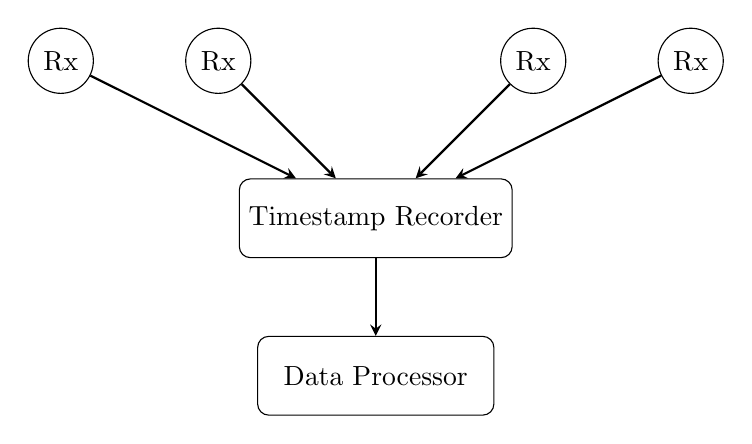
\begin{tikzpicture}[node distance=2cm]
%\node (tx) [draw=none, circle]                 {};
%\draw (tx) circle (0.9);
%\draw (tx) circle (1.3);

%--------- Receivers ---------%
%\node (rx1) [draw, circle, below of = tx]  {Rx};
\node (rx1) [draw, circle               ]  {Rx};
\node (rx2) [draw, circle, right of = rx1] {Rx};
\node (CTR) [rectangle, draw=none, right of = rx2] {};
\node (rx3) [draw, circle, right of = CTR] {Rx};
\node (rx4) [draw, circle, right of = rx3] {Rx};

%--------- Devices ---------%
\node (arduino) [device, below of = CTR] {Timestamp Recorder};
\node (pi) [device, below of = arduino] {Data Processor};

%--------- Arrows ---------%
\draw [arrow] (rx1) -- (arduino);
\draw [arrow] (rx2) -- (arduino);
\draw [arrow] (rx3) -- (arduino);
\draw [arrow] (rx4) -- (arduino);
\draw [arrow] (arduino) -- (pi);

\end{tikzpicture}
\end{center}
\caption{A simple diagram detailing the main components.
	Each circle labeled Rx is a receiver, consisting of a piezoelectric
	transducer and some processing circuitry.}
\label{fig:component-diagram}
\end{figure}

For a more detailed version of this figure, see the
Wiring Diagram (\ref{fig:wiring}) in Section \ref{sec:wiring}.

%%%%%%%%%%%%%%%%%%%%%%%%%%%%%%%%%%%%%%%%%%%%%%%%%%%%%%%%%%%%%%%%%%%%%%%%%%%%%%%
\section{Electronics Hardware}\label{sec:ee-hardware}

While both the Arduino and the Raspberry Pi were off-the-shelf products,
the transmitter and receiver hardware was all custom designed and fabricated
for use in this project.
Clearer specifications, including detailed diagrams, are given in other
dedicated documents, so the information presented here will only be a
high-level overview of the main components.

\subsection{Transmitters}

The transmitters are small piezoelectric transducers that oscillate at an
ultrasonic frequency.
In our work, this frequency has been in the 40-60kHz range, depending on the
resonant frequency of the transducer itself.
Though we have not established bounds on our range of potential frequencies,
the actual frequency that is selected shouldn't matter so long as all of the
hardware is capable of operating at, and
appropriately tuned to, the frequency (through filtering,
hardware characteristics, and so on).
For example, some hardware may limited to roughly 150kHz because the
microcontrollers won't have a high enough clock speed to drive
the receivers at that rate.

Each transmitter is attached to a small \gls{pcb} designed
specifically for the project.
The \gls{pcb} can power the transducer by feeding it a current, effectively
turning it off or on as needed.
Each board will be programmed with a unique identifier (a numeric value).
The ID determines the pattern of pulses that the transmitter should emit.
For more details on this, see the \gls{iCRAB-proto} document.

\subsection{Receivers}

The receivers include small piezoelectric transducers that are able to detect
vibrations in the same range as the transmitters.
A preamplifier steps up the signal from the transducer before sending this
signal along to a band-pass filter.
The band-pass filter restricts the frequencies that the hardware will
detect, meaning that a lot of irrelevant noise can be discarded.
After being filtered, the signal is then amplified.
A potentiometer on the board allows for variable amplification.
Next, the signal is
rectified (effectively producing the absolute value of the incoming sine wave).
The low pass filter transforms the signal from a sinusoidal wave into a single
pulse.
Finally, the Schmitt Trigger acts as a variable threshold, preventing a noisy
rising or falling edge from being interpreted as a series of short rising and
falling edges.
See Figure \ref{fig:rx-detail} for details on this pipeline.

\begin{figure}[h]
\begin{center}
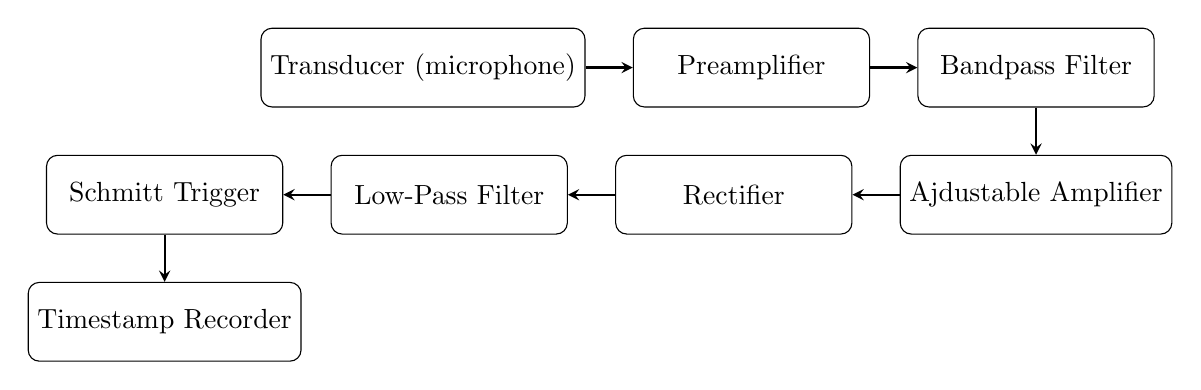
\begin{tikzpicture}[node distance=0.6cm]

\node (mic)    [device]                    {Transducer (microphone)};
\node (preamp) [device, right = of mic]    {Preamplifier};
\node (bp)     [device, right = of preamp] {Bandpass Filter};

\node (adjamp) [device, below = of bp]    {Ajdustable Amplifier};
\node (rect)   [device, left = of adjamp] {Rectifier};
\node (lowp)   [device, left = of rect]   {Low-Pass Filter};
\node (schmt)  [device, left = of lowp]   {Schmitt Trigger};

\node (ard)    [device, below = of schmt] {Timestamp Recorder};

\draw [arrow] (mic) -- (preamp);
\draw [arrow] (preamp) -- (bp);
\draw [arrow] (bp) -- (adjamp);
\draw [arrow] (adjamp) -- (rect);
\draw [arrow] (rect) -- (lowp);
\draw [arrow] (lowp) -- (schmt);
\draw [arrow] (schmt) -- (ard);

\end{tikzpicture}
\end{center}
\caption{The receiver hardware pipeline.}
\label{fig:rx-detail}
\end{figure}

The resulting digital signal is sent over a wire to the timestamp
recorder detailed in section \ref{sec:ts-rec}.

%%%%%%%%%%%%%%%%%%%%%%%%%%%%%%%%%%%%%%%%%%%%%%%%%%%%%%%%%%%%%%%%%%%%%%%%%%%%%%%
\section{Computer Hardware}\label{sec:cs-hardware}

Signals detected through the receiving hardware described in
Section \ref{sec:ee-hardware} are delivered to more advanced microcontrollers
and computers using common \gls{gpio} pins.
Two separate devices are used for the signal processing.
The first,
referred to in this document as the Timestamp Recorder (\ref{sec:ts-rec}),
provides a
low-latency means of detecting the time of an incoming signal.
This device must be able to reliably detect when a signal arrives with
sub-millisecond precision.
Once timestamped, the data can be transferred to the
Data Processor (\ref{sec:data-processor}).
This device decodes the ID from each transmission and displays the crab's
direction to the user.

\subsection{Timestamp Recorder}\label{sec:ts-rec}

The timestamp recorder reads a digital signal on a \gls{gpio} pin and records
the ``time'' at which the signal changed from low to high or vice versa.
In this case, the ``time'' need not have any meaningful relationship to
``wall clock'' time, so long
as the timestamps have some meaning relative to each other.
For example, the time associated with a state change could be measured in
microseconds since the board reset.
Since the software (described in Section \ref{sec:sw-data-proc}) is primarily
concerned with the time separation between events, the epoch is irrelevant.
It is important, however, that the Timestamp Recorder and the Data Processor
computers agree on the units used, because some of the later processing will be
based on the speed of sound in water, measured in meters per second.

In addition to providing reliable timing measurements when input pin states
change, the timestamp recorder must also be able to communicate the timestamped
data to another device.
Use of a non-blocking protocol such as \gls{spi} is
necessary here so that the data transfers do not have a large negative impact
on the device's ability to continuously detect changes.

\subsection{Data Processor}\label{sec:data-processor}

The majority of the processing software exists on a separate device, referred
to as the Data Processor.
This machine reads timestamped data from the
Timestamp Recorder (\ref{sec:ts-rec}) and stores it in its own local storage
until it has enough data to run some calculations.
This device is also the user's primary interface for interacting with the
system in most use cases.
Equipped with a touchscreen or other means of displaying data, the computer is
able to display the unique identification numbers and relative locations of
crabs as they are detected.

The software written for this project assumes that the Data Processor is a
Linux-based machine with an \gls{spi} interface.
Specifically, it has been tested on a Raspberry Pi 3B, which is a very
suitable device given its low cost, built-in \gls{gpio} pins, and adequate
processing power.

\subsection{Wiring Diagram}\label{sec:wiring}

This section demonstrates in greater detail how the various components are
connected to each other.
Note that though we use the official 7" touchscreen built for the Pi,
wiring for the screen is not included in the following diagram.
In Figure \ref{fig:wiring}, the Pi (the SPI master node),
Arduino (SPI slave node), and a receiver are shown.
Note that each of the other receivers could be connected in the same way
that Receiver 1 is connected; that is, they need to be tied to the common
ground and they need their signal pin attached to the appropriate input pin
on the Arduino.

\begin{figure}[h]
\begin{center}
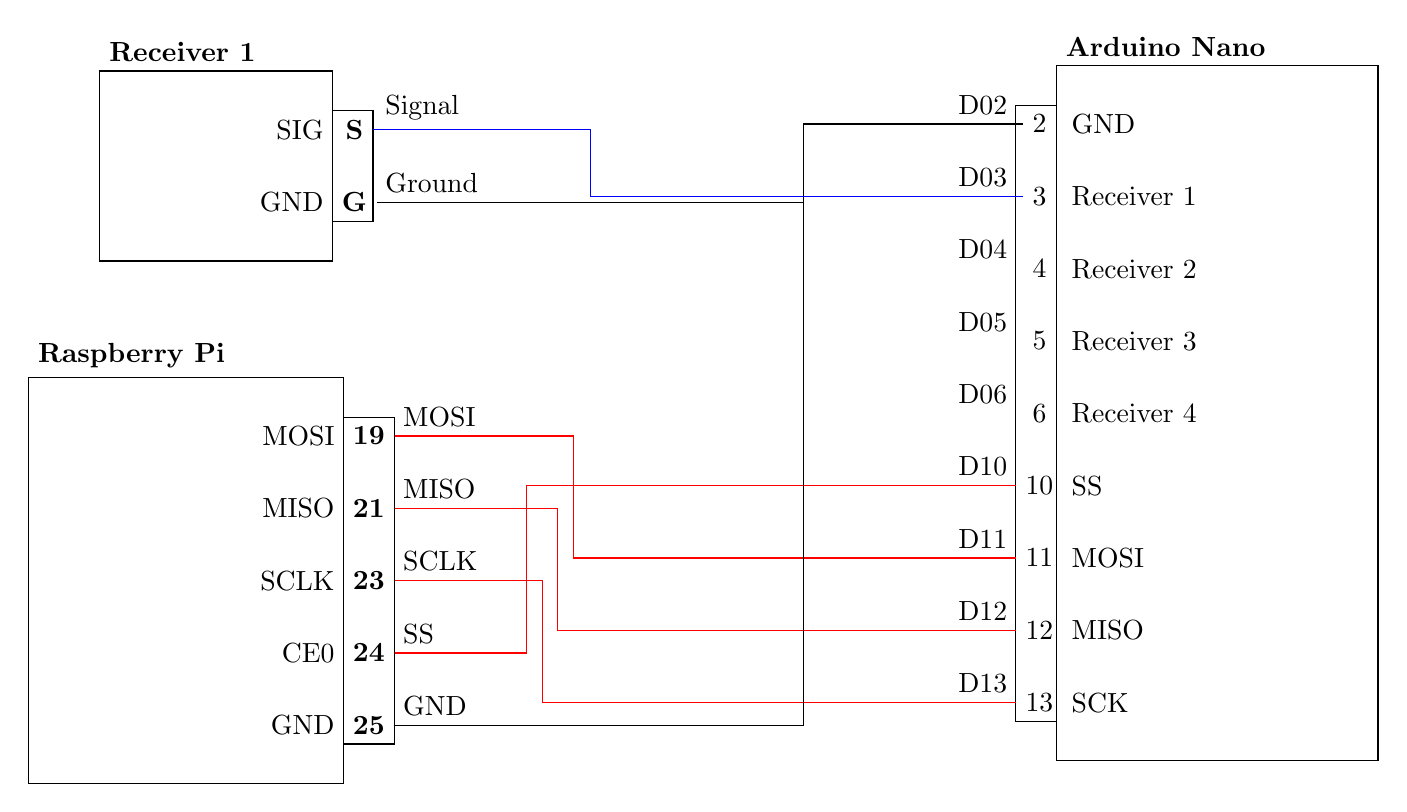
\begin{tikzpicture}

% Pinout diagram based on:
% https://tex.stackexchange.com/questions/241357/wiring-diagrams-with-pinout

%%%%%%%%%%%%%%%%%%%%%%%%%%%%%%%%%%%%%%%
% Pins and labels on devices
%%%%%%%%%%%%%%%%%%%%%%%%%%%%%%%%%%%%%%%

\matrix[wire board,rx](Rx1){
	SIG   & S & Signal  \\
	GND   & G & Ground  \\
};

\matrix[wire board,pi, matrix anchor=north, below = 2cm of Rx1.south](Pi){
	MOSI  & 19 & MOSI  \\
	MISO  & 21 & MISO  \\
	SCLK  & 23 & SCLK  \\
	CE0   & 24 & SS    \\
	GND   & 25 & GND  \\
};

\matrix[wire board,arduino, matrix anchor=north, right = 9cm of Rx1.north] (Arduino){
	D02 &  2 & GND           \\
	D03 &  3 & Receiver 1    \\
	D04 &  4 & Receiver 2    \\
	D05 &  5 & Receiver 3    \\
	D06 &  6 & Receiver 4    \\
	D10 & 10 & SS    \\
	D11 & 11 & MOSI  \\
	D12 & 12 & MISO  \\
	D13 & 13 & SCK   \\
};

%%%%%%%%%%%%%%%%%%%%%%%%%%%%%%%%%%%%%%%
% Boxes around devices
%%%%%%%%%%%%%%%%%%%%%%%%%%%%%%%%%%%%%%%

% Add boxes around Rx1
\draw (Rx1-1-2.north east) rectangle (Rx1-2-2.south west);
\draw (Rx1-1-2.north west)+(-3cm,0.5cm)
	node[above right, font=\bfseries]
	{Receiver 1}
	rectangle
	($(Rx1-2-2.south west)+(0,-0.5cm)$);

% Add boxes around Pi
\draw (Pi-1-2.north east) rectangle (Pi-5-2.south west);
\draw (Pi-1-2.north west)+(-4cm,0.5cm)
	node[above right, font=\bfseries]
	{Raspberry Pi}
	rectangle
	($(Pi-5-2.south west)+(0,-0.5cm)$);

% Add boxes around Arduino
\draw (Arduino-1-2.north east) rectangle (Arduino-9-2.south west);
\draw (Arduino-1-2.north east)+(0cm,0.5cm)
	node[above right, align=center, font=\bfseries]
	{Arduino Nano}
	rectangle
	($(Arduino-9-2.south east)+(4cm,-0.5cm)$);

%%%%%%%%%%%%%%%%%%%%%%%%%%%%%%%%%%%%%%%
% Wires between devices
%%%%%%%%%%%%%%%%%%%%%%%%%%%%%%%%%%%%%%%

% SPI connections
\draw[color=red]
	(Pi-1-2) -- +(2.60cm,0) |- (Arduino-7-2) % MOSI
	(Pi-2-2) -- +(2.40cm,0) |- (Arduino-8-2) % MISO
	(Pi-3-2) -- +(2.20cm,0) |- (Arduino-9-2) % SCLK
	(Pi-4-2) -- +(2.00cm,0) |- (Arduino-6-2) % SS
;

% Shared Ground
\draw
	(Arduino-1-2) -- +(-3cm,0) |- (Pi-5-2)
	(Arduino-1-2) -- +(-3cm,0) |- (Rx1-2-2)
;

\draw[color=blue]
	(Rx1-1-2) -- + (3cm,0) |- (Arduino-2-2)
;

\end{tikzpicture}
\end{center}
\caption{A wiring diagram for the devices at the receiving station.}
\label{fig:wiring}
\end{figure}

\gls{spi} uses four shared wires. Briefly, the purpose of each is:
\begin{itemize}
\item \texttt{MOSI} Master-In-Slave-Out -- data from the slave to the
	master (such as timestamps and pin values).
\item \texttt{MISO} Master-Out-Slave-In -- data from the master to the
	slave (used for flags, in our case).
\item \texttt{SCLK} The clock. Driven by the master node.
\item \texttt{SS} or \texttt{CE} is the Slave Select or Chip Enable line.
	\gls{spi} supports multiple slave devices, so the master node uses
	the Chip Enable line to turn on one slave at a time to communicate.
	In our case, since there is only one slave device, we know that the
	\texttt{CE0} line will always be active during a transfer.
\end{itemize}


%%%%%%%%%%%%%%%%%%%%%%%%%%%%%%%%%%%%%%%%%%%%%%%%%%%%%%%%%%%%%%%%%%%%%%%%%%%%%%%
\section{Software}\label{sec:software}

Wherever possible, the software for this project was written in such a way that
various elements may be altered or entirely replaced without requiring major
changes to the rest of the codebase.
The hope is that it is flexible enough to be adapted for new scenarios and
hardware setups in the future.
That said, it has only been tested with the hardware detailed elsewhere in this
document, so its portability and modularity is unproven.

In this section, we will examine the software that runs on the two devices
described in Section \ref{sec:cs-hardware}.

\subsection{Timestamp Recorder Software}\label{sec:ts-rec-sw}

The relevant source code can be found here:
\texttt{src/arduino-src/arduino-src.ino} in the project source or on
\href{https://github.com/cabeese/crab-tracker/tree/master/src/arduino-src}
{GitHub}.


The Timestamp Recorder (\ref{sec:ts-rec}) software has two primary functions:
(1) record timestamps of signal changes (i.e. when a pin goes high or low) and
(2) transfer the timestamps and pin values to the Data Processor.

The \texttt{arduino-src.ino} file is heavily documented, so this section
will explore the major ideas without providing extensive detail about
individual lines.
Specifically, it will examine in broad strokes the data formatting, data
transfer, and input pin change detection.

\subsubsection{Storage, Setup and Loop}

Data is stored in a bounded buffer where each entry contains a timestamp value
and the state of the pins at that timestamp (i.e. which pins were high and
which were low).
The timestamp is a 32-bit \texttt{unsigned long} and the pin values are
all stored in a single \texttt{byte} where each bit corresponds to a single
pin.
The \texttt{pinvals} are shifted such that the lowest order bit corresponds
to pin D3.
A 1 in position 0 means that pin D3 is high; 0 means low.
(Note that a few of the low-order pins on the board are reserved for special
purposes, so the receivers are to be attached to pins D3 through D6.)

The \texttt{setup()} function sets the \gls{gpio} pins on Port D (pins 0-7)
as input pins, meaning that another device (in this case, a receiver, as
described in section \ref{sec:ee-hardware}) can drive the line high or low.
The Timestamp Recorder can detect these changes when the pins are in input
mode.

The \texttt{loop()} function runs indefinitely and on each iteration it can fill
the \gls{spi} data register and/or detect and timestamp a change on one of the
pins.
We will examine both of these primary functions in more detail in the following
two sections.

\subsubsection{SPI Handling}

\gls{spi} is a synchronous serial communication interface that is natively
supported by both the Arduino and the Raspberry Pi.
It supports a single ``master'' node and multiple ``slave'' nodes.
When the master node is ready to transfer data, it selects one of the
slave devices by making its Chip Enable/Slave Select line active and then
begins pulsing the clock.
More details about the \gls{spi} protocol can be found online.

The Arduino Nano has a built-in \gls{spi} bus that supports 8-bit data
transfers.
On a transfer, the master node provides a clock pulse and on every pulse, one
bit is shifted out of the data register (sent to the master) and one bit is
shifted in (sent from the master).

On each iteration of the loop, the Arduino checks to see if the ``End of
Transmission'' flag is set, which indicates that a transfer has completed.
If it is set, the board can fill the Data Register with the next byte to be
sent.
The next time the master requests data, the newly-loaded byte will be shifted
out to that device.

As mentioned, the built-in \gls{spi} hardware supports 8-bit data transfers.
However, each segment of data that we wish to transfer contains a 32-bit
timestamp and an 8-bit state, meaning that it takes 5 individual transfers
to send a segment (or ``block'') of data.
When the master node requests data, the slave sends the pin values on the
first transfer, and then sends the timestamp in 8-bit chunks over the course of
the next four transfers, starting with the lowest order byte and working up to
the highest order byte.
Note that this means both the master and slave nodes must be in sync with
each other, as there is nothing to indicate what kind of data is sent in a
single transfer.
The two devices may get out of sync if one is interrupted between transfers,
such as when the master's software is stopped unexpectedly.
In this case, when the master's software restarts, it will expect to read
pin values on the first transfer, even though the slave node may be prepared
to send part of a timestamp.

To solve this issue, the \gls{spi} master node can send flags to the slave
that will alter the slave's state or behavior.
Certain values that the master can send will induce specific behaviors on the
slave.
For example, the \texttt{SPI\_ECHO\_REQUEST} flag, when sent, will cause the
slave to send the \texttt{SPI\_ECHO\_RESPONSE} value on the next transfer.
This is used when the master's program starts up in order to ensure that the
two devices are correctly connected.
The \texttt{SPI\_RESET} flag will re-position the de-facto ``read heads'',
meaning that it will send a new state starting with the pin values on the next
transfer.
This functionality is utilized to ensure that the two devices stay in sync when
one of them restarts while the other continues to run.

%\begin{figure}[h]
%\begin{center}
%\begin{tikzpicture}[shorten >=1pt,node distance=2cm,on grid]
%%\tikzstyle{every state}=[draw=none, text=white]
%
%\node[initial,state] (pinvals)                    {pinvals};
%\node[state]         (ts-0)    [right=of pinvals] {ts [0..7]};
%\node[state]         (ts-1)    [right=of ts-0]    {ts [8..15]};
%\node[state]         (ts-2)    [right=of ts-1]    {ts [16..23]};
%\node[state]         (ts-3)    [right=of ts-2]    {ts [24..31]};
%
%\path[->] (pinvals) edge    node {} (ts-0)
%          (ts-0)    edge    node {} (ts-1)
%          (ts-1)    edge    node {} (ts-2)
%          (ts-2)    edge    node {} (ts-3)
%          (ts-3)    edge [bend left=45]   node [above] {} (pinvals)
%;
%
%\end{tikzpicture}
%\end{center}
%\caption{The state machine for SPI transfers.}
%\label{fig:spi-state-machine}
%\end{figure}

\subsubsection{Pin Change Detection and Timestamping}

Pin change detection is comparatively straightforward.
Each time the loop runs, the current state of the relevant pins (D3..D6) is
compared with the state recorded from the previous iteration.
If the two states differ, this indicates that at least one pin changed from
low to high or vice versa.
When this is the case, the device stores the new state in a circular
buffer along with the current time.

As of the current revision of the document, the timestamp is generated from
the \texttt{TCNT0} clock, which increments every four microseconds.
This is an inadequate granularity for the purposes of this project, so future
revisions of the code will instead read from a source that can generate ticks
at a higher rate (for example, a clock cycle counter, or a timer set up to
increment once every microsecond).

Note that no matter the units used, we should expect to store no more than 32
bits of information for any given timestamp.
Therefore, $2^{32} \approx 4.3$ million is the highest value we can represent.
Limited precision means that a source that increments frequently will overflow
more rapidly than a slower source, which leads to an important trade-off.
A 4-millisecond timer will overflow every $4\times (4.3\times 10^6)$
milliseconds, or roughly once every 4,772 hours.
However, a timer that increments once per microsecond will overflow every 1.1
hours (or roughly 72 minutes).
Currently, overflowing timer values are not handled by any part of the
software; instead, any such data will automatically be thrown out.
In other words, if a transmission is received while an overflow occurs, such
that some timestamps have extremely high values while others have extremely
low (near-0) values, that transmission will be ignored.
No attempt is made to account for the overflow, though to do so is well within
the realm of possibility for future work.

\subsection{Data Procesesor Software}\label{sec:sw-data-proc}

The relevant source code can be found in multiple files in
\texttt{src/pi-src/} in the project source or on
\href{https://github.com/cabeese/crab-tracker/tree/master/src/pi-src}{GitHub}.

\subsubsection{Overview of Files}

The primary functions of the various files are as follows:
\begin{itemize}
\item \texttt{main.cpp} --
	The main loop of the program. This file periodically polls the
	\gls{spi} slave device and then runs routines to process any data that
	is fetched.
\item \texttt{data\_collection.cpp} --
	When SPI data is read, the functions in this file parse and store the
	data in meaningful structures.
	For example, when a rising and subsequent falling edge are detected on a
	given pin, a \texttt{ping} object is stored containing these timestamps.
	The data collection code also steps through the collected data to determine
	if enough pings have been collected for the direction algorithm to run.
	For more details, see Section \ref{sec:proc-and-structure}.
\item \texttt{direction.cpp} --
	Using an algorithm written by one of the team's developers, Chloe Yugawa,
	this code determines the relative direction of a crab given the timestamps
	of its pings.
	That is, it performs a Time Difference On Arrival calculation
	based on ping times.
	It returns a direction relative to the front of the boat in cylindrical
	coordinates in the form $(r, \theta, z)$.
	For more information, see the
	Triangulation Algorithm$^{\ref{ref-dir-alg}}$ document.
\item \texttt{spi.cpp} --
	This file facilitates and abstracts away the communication with the
	\gls{spi} slave device.
	Routines in this file can determine if the devices are properly connected
	and will also ensure that the master and slave devices are in
	sync with each other.
\item \texttt{uid.cpp} --
	Each transmitter broadcasts in a specific pattern based on its unique
	identifier. The code in this file examines the duration of and delay
	between two pings and determines the UID(s) that these time values
	encode.
\item \texttt{util.cpp} --
	Various helper methods are located here, including binary printing
	functions and configuration setting loading.
\item \texttt{/etc/crab-tracker.conf} --
	Configuration options are located in this file in the \texttt{/etc}
	directory. Data is stored in key/value pairs and is read on program
	startup. Parameters include what kind of data should be logged, the
	distance between the corners of the hydrophone array, and more.
\end{itemize}

\subsubsection{Processing and Structure}\label{sec:proc-and-structure}

Each file contains extensive documentation, so the finer details about
various functions and variables will not be
duplicated in this document. Instead, we'll take a broad look at how these
pieces fit together.

When data is read from the Timestamp Recorder, it is translated from raw pin
states into something more meaningful, such as a ``ping'' (that is, a single
broadcast as measured by the rising and falling edges of a signal on a single
pin).
Pings are collected in a set of buffers, with one buffer for each pin.
These buffers are managed by the \texttt{data\_collection.cpp} code.
Since the \gls{iCRAB-proto} mandates that every transmission consists
of two pings, no calculations are performed until a pair of pings is detected
by all four receivers.
Each time a new ping is detected, these arrays are searched for matching pairs.
If there are two pings in every buffer, and they all share the same ID
and are spaced apart correctly (temporally, based on \gls{iCRAB-proto}
specifications), they are all returned as a set of 8 pings to the main loop of
the program, which then runs the direction calculation algorithm.
If the direction algorithm is able to determine an approximate location for
the signal$^*$, the direction and associated ID can be reported to the user.

\vfill
$^*$ Note that the direction algorithm will intentionally fail if it is given
impossible data.
That is, if the timestamps are too widely separated temporally, it will assume
that the measurements are not from the same transmission or are otherwise
incorrect and will therefore abort the direction calculation.

%%%%%%%%%%%%%%%%%%%%%%%%%%%%%%%%%%%%%%%%%%%%%%%%%%%%%%%%%%%%%%%%%%%%%%%%%%%%%%%
\newpage

\section{References} \label{references}

Unless otherwise noted, the documents referenced in this section are published
\href{https://github.com/cabeese/crab-tracker/tree/master/doc}{on GitHub},
or else in the same location as this PDF.

\begin{enumerate}
\item \label{ref-icrab-proto}
        Strong, N.
        {\em Transmission Protocol -- iCRAB.}
        2018. PDF.
\item \label{ref-rfc1}
        Strong, N.
        {\em RFC 1: Collisions in Delay-Based ID Encoding Protocol.}
        2017. PDF.
\item \label{ref-rfc2}
        Strong, N.
        {\em RFC 2: Boolean Value Encoding in Transmission Protocol.}
        2018. PDF.
\item \label{ref-rfc-stats}
        Yugawa, C.
        {\em RFC Stats.}
        2017. PDF.
\item \label{ref-dir-alg}
        Yugawa, C.
        {\em Triangulation Algorithm.}
        2017. PDF.
\end{enumerate}


\printglossary

\end{document}

